\documentclass[12pt]{beamer}

% \usepackage{cmap}
\usepackage[english, russian]{babel}

\usetheme{metropolis}
\usepackage{appendixnumberbeamer}

\usepackage{booktabs}
\usepackage{minted}
\usepackage[many]{tcolorbox}
\usepackage{mdframed}

\usepackage{listings}
\lstset{basicstyle=\ttfamily\small,
	showstringspaces=false,
	breaklines=true,
	frame=lrtb,
	% numbers=left,
	extendedchars=\true,
	language=Java
}

\usepackage{xcolor}

\usepackage{xspace}
\newcommand{\themename}{\textbf{\textsc{metropolis}}\xspace}
% \setsansfont{Fira Sans Bold}

% \surroundwithmdframed{minted}

\title{Автоматизация миграции программного кода на новый набор библиотек}
% \subtitle{A modern beamer theme}
\date{\today}
\author{Артем Алексюк}
\institute{Санкт-Петербургский политехнический университет Петра Великого \\
JetBrains Research}
\titlegraphic{\hfill
\includegraphics[height=1.5cm]{WIP.png}}

\newtcolorbox{mybox}[1][]{
    width=\textwidth,
    arc=3mm,
%    auto outer arc,
    boxsep=0cm,
    toprule=1pt,
    leftrule=1pt,
    bottomrule=1pt,
    rightrule=1pt,
    colframe=white,
    boxrule=0pt,frame hidden,
    breakable,
    nobeforeafter,
    enhanced jigsaw,
    opacityframe=0.7,
    fontupper=\bfseries,
    opacityback=0.7
}

\setbeamercolor{itemize/enumerate body}{fg=black}

% \setbeamertemplate{blocks}[rounded][shadow=false]
% \addtobeamertemplate{block begin}{\pgfsetfillopacity{0.5}}{\pgfsetfillopacity{1}}

\begin{document}

\maketitle

%\begin{frame}{Table of contents}
%  \setbeamertemplate{section in toc}[sections numbered]
%  \tableofcontents[hideallsubsections]
%\end{frame}

% \section{Introduction}


{
\usebackgroundtemplate{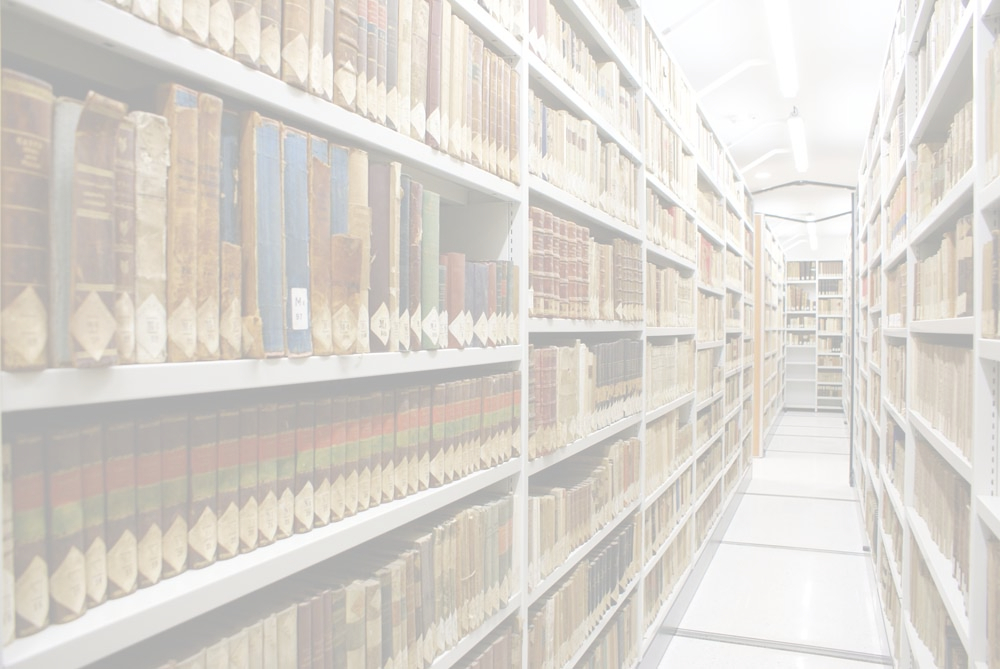
\includegraphics[height=\paperheight,width=\paperwidth]{historical-archive.jpg};}
\begin{frame}{Актуальность}
\begin{mybox}[]
Миграция (портирование) в новое библиотечное окружение:
\begin{itemize}
	\item Новая программная платформа
	\item Новая аппаратная платформа
	\item Новая версия библиотеки
	\item Унаследованный (несовместимый) код 
	\item ...		
\end{itemize}
\end{mybox}
\end{frame}
}

{
\usebackgroundtemplate{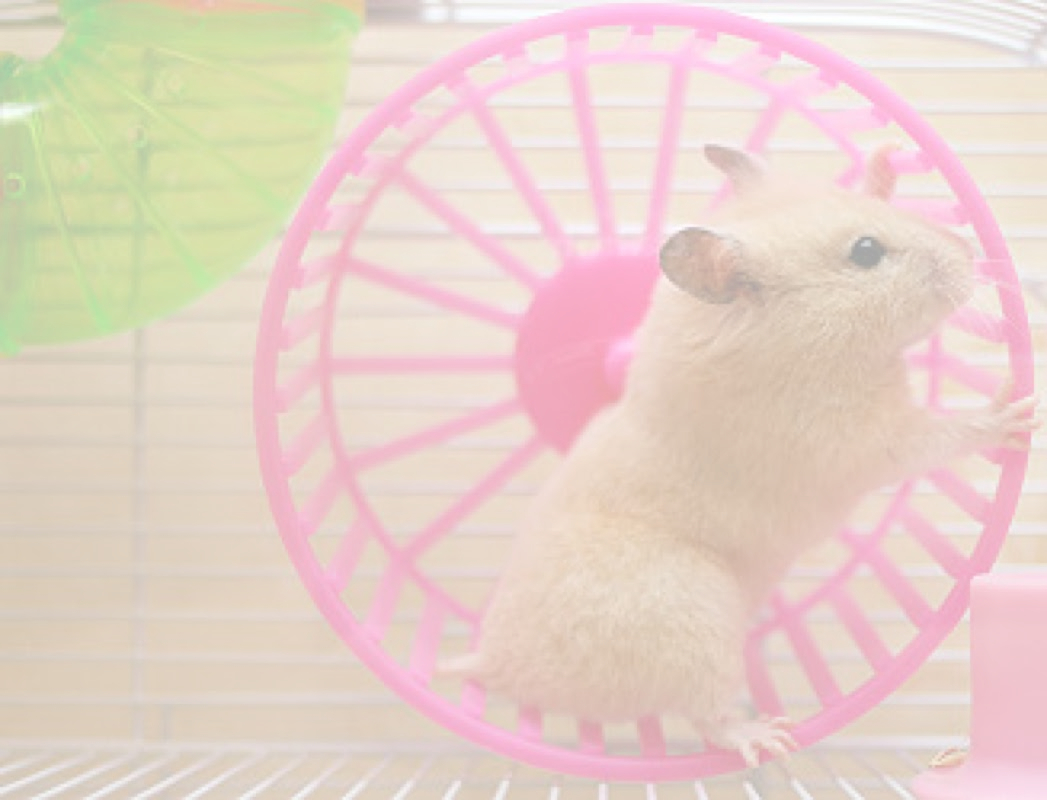
\includegraphics[width=\paperwidth]{wheel3.jpg};}
\begin{frame}{Сложности}
\begin{mybox}[]
\begin{itemize}
	\item Практически всегда миграция идет вручную
	\item Много рутинной работы $\Longrightarrow$ высокая вероятность внесения ошибок
	\item Однотипные действия при миграции нескольких проектов
\end{itemize}
\end{mybox}
\vspace{0.5cm}
\begin{mybox}[]
\begin{center}
    Требуется автоматизация
\end{center}
\end{mybox}
\end{frame}
}

\begin{frame}[fragile]{Пример задачи миграции}
	Программа, использующая библиотеку java.net.URLConnection:
\begin{minted}[breaklines,fontsize=\small]{java}
URL url = new URL("http://api.ipify.org/");
URLConnection conn = url.openConnection();
\end{minted}
	Программа, использующая библиотеку Apache HttpClient:
\begin{minted}[breaklines,fontsize=\small]{java}
CloseableHttpClient httpclient = HttpClients.createDefault();
HttpGet httpget = new HttpGet("http://api.ipify.org/");
CloseableHttpResponse httpResponse = httpclient.execute(httpget);
\end{minted}
\end{frame}

\begin{frame}{Общая схема решения задачи}
\begin{center}
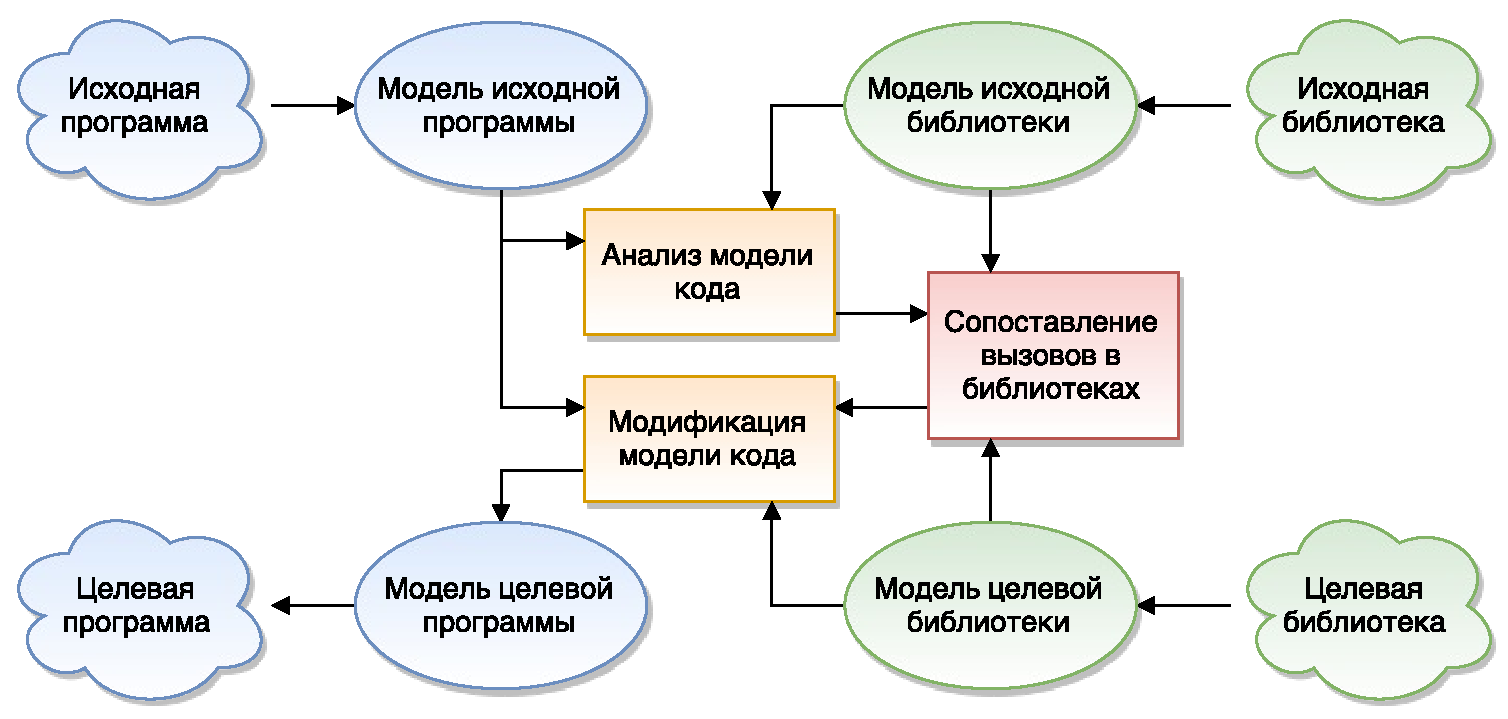
\includegraphics[width=\textwidth]{scheme.pdf}
\end{center}
\end{frame}

%{
%\usebackgroundtemplate{%
%\tikz\node[opacity=0.4]{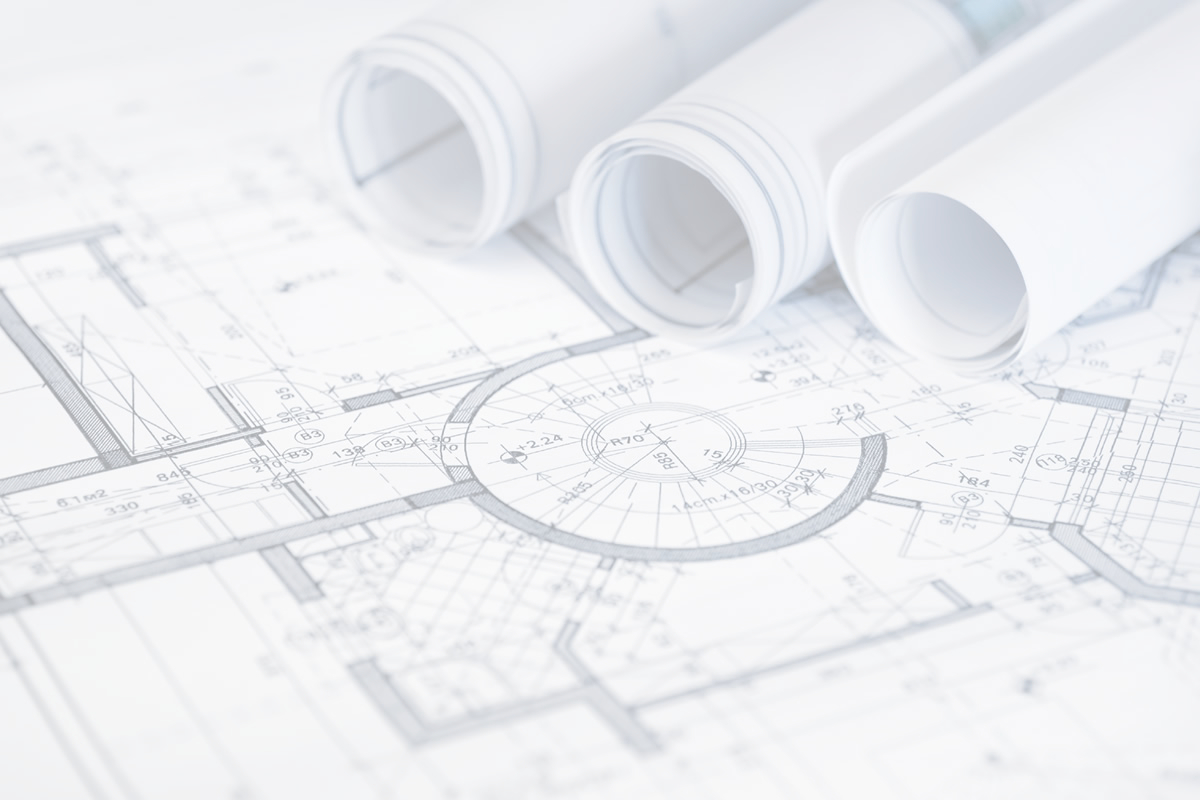
\includegraphics[height=\paperheight,width=\paperwidth]{spec.jpg}};}
%\begin{frame}{Модели библиотек}
%\begin{mybox}[]
%	Модель библиотеки должна:
%\begin{itemize}
%	\item Детально описывать внешний интерфейс библиотеки
%	\item Задавать возможные протоколы использования библиотеки;
%	\item Специфицировать побочные действия библиотеки – влияние ее на окружение;
%\end{itemize}
%\end{mybox}
%\end{frame}
%}

{
\usebackgroundtemplate{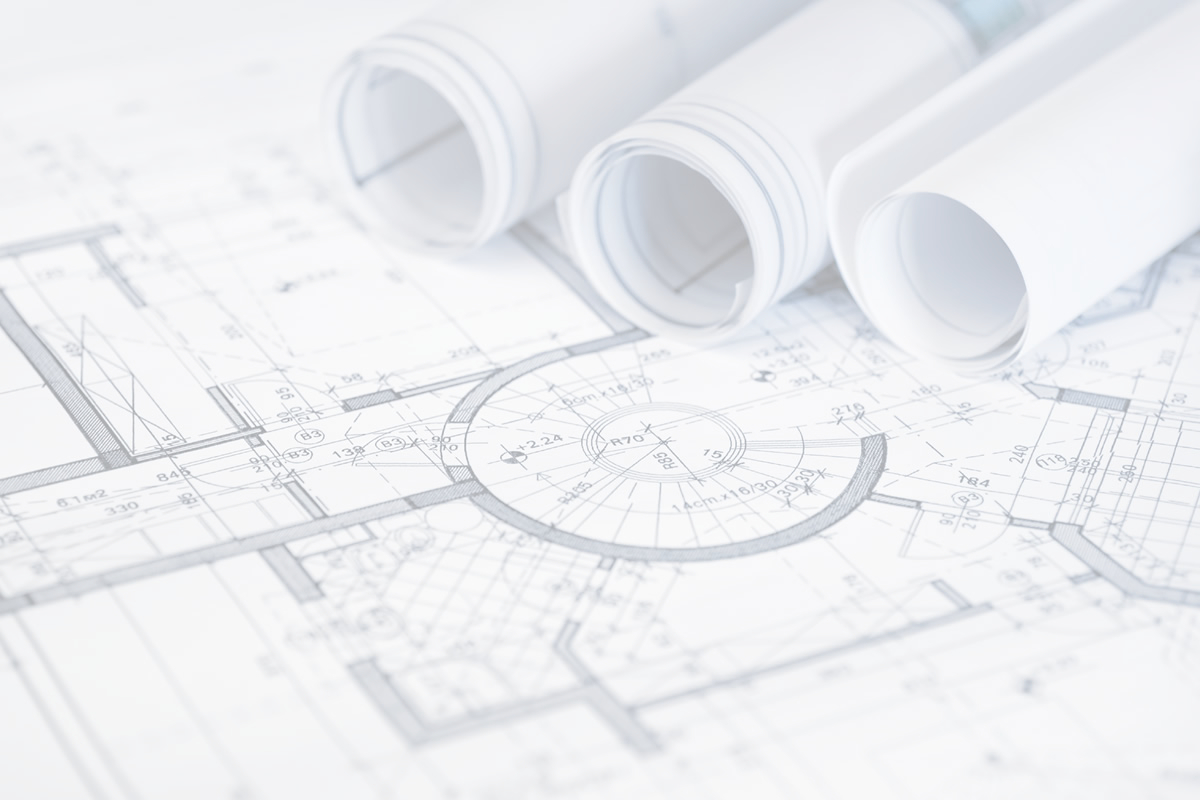
\includegraphics[height=\paperheight,width=\paperwidth]{spec.jpg};}
\begin{frame}{Модель библиотеки}
  \begin{mybox}[]
  Для описания моделей используется набор расширенных конечных автоматов
  \begin{itemize}
  	\item Каждый переход в автомате --- действие над библиотекой
  	\item В процессе перехода могут порождаться новые автоматы
  	\item Автомат может иметь атрибуты, и переходы могут зависеть от них
  	\item Для переходов можно указать их побочные эффекты
  \end{itemize}
  \noindent\rule{4cm}{0.4pt}
  
  \begingroup
  \tiny
    	Ицыксон В.М. Формализм для спецификации семантики программных библиотек. 2016 г.
  \endgroup
  \end{mybox}
\end{frame}
}

% \section{Titleformats}

\begin{frame}{Пример автомата}
\begingroup
\scriptsize
* Иллюстрации сгенерированы автоматически
\endgroup
\begin{center}
	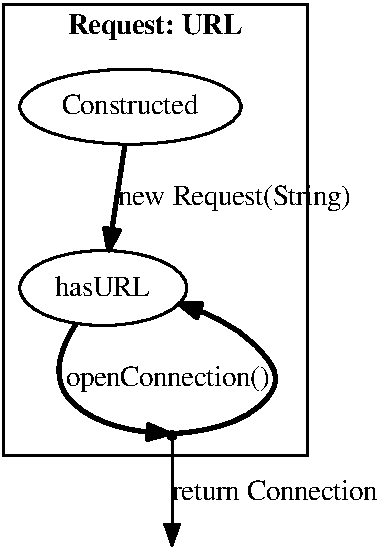
\includegraphics[height=0.8\textheight]{javaSmall-cropped.pdf}
\end{center}
\end{frame}

\begin{frame}{Фрагмент модели библиотеки URLConnection}
\begin{center}
	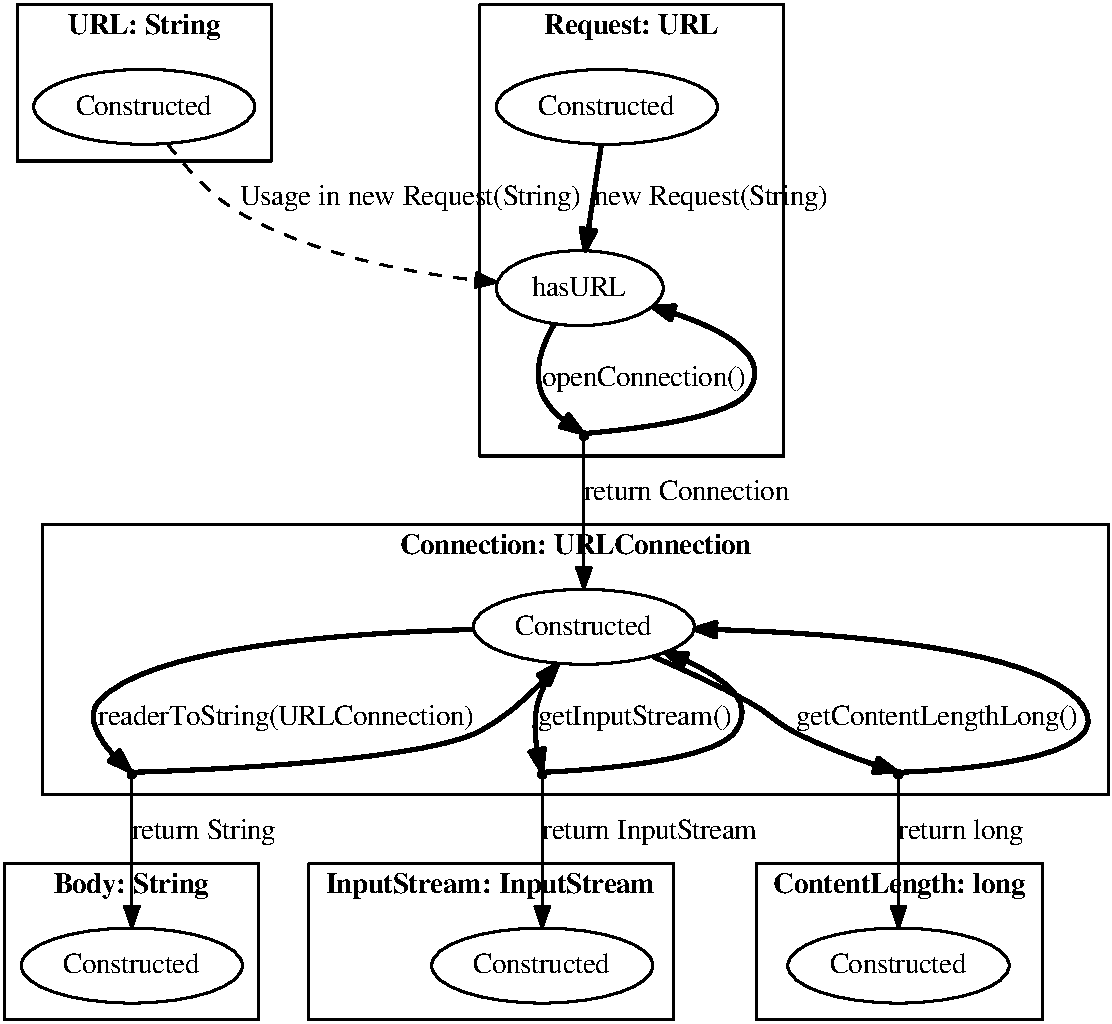
\includegraphics[width=0.75\textwidth]{java-cropped.pdf}
\end{center}
\end{frame}

\begin{frame}{Фрагмент модели библиотеки Apache HttpClient}
\begin{center}
	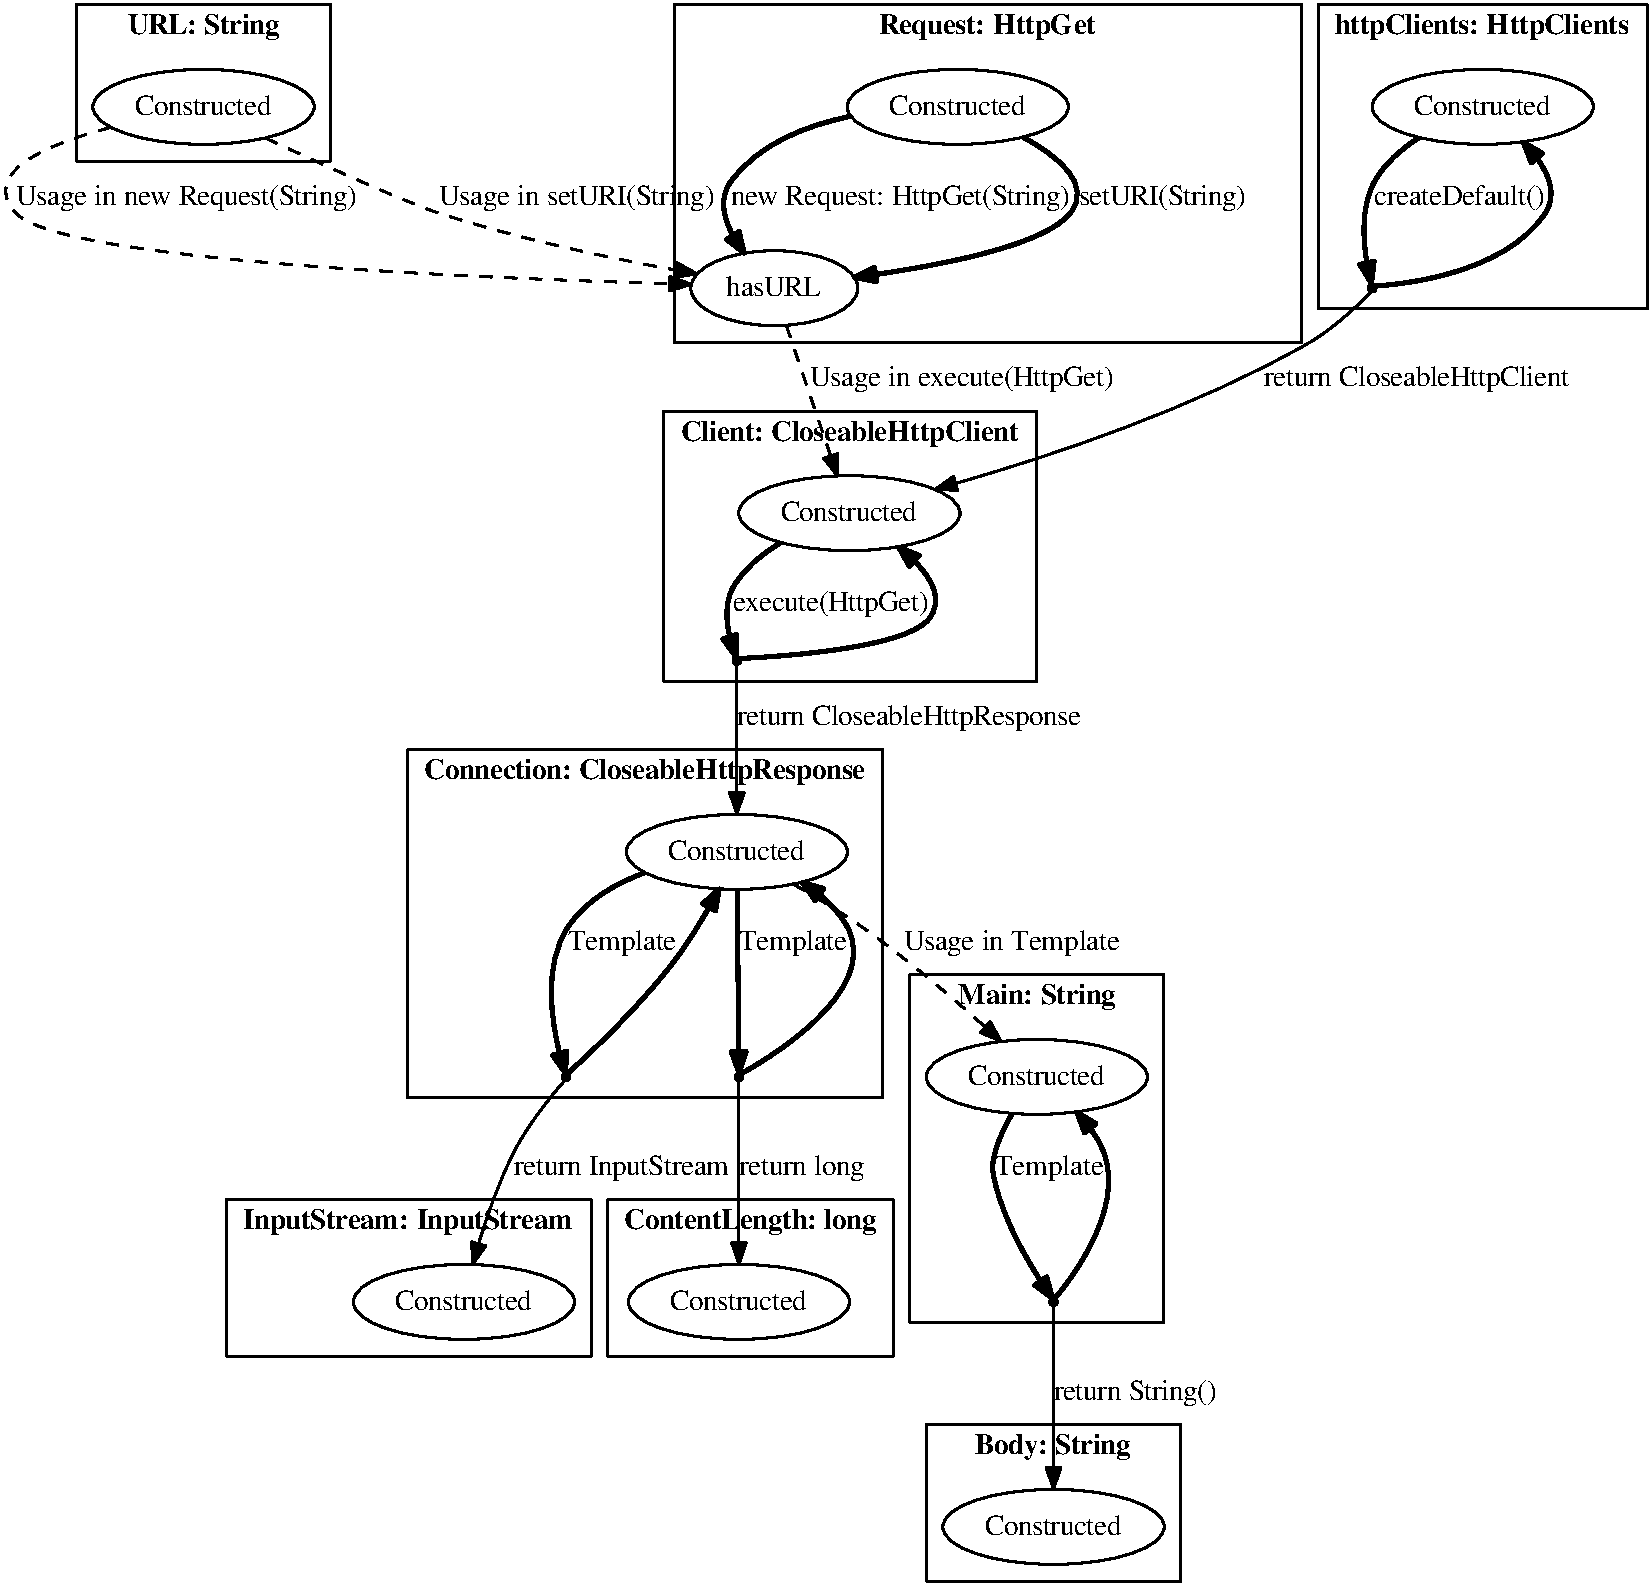
\includegraphics[width=0.7\textwidth]{apache-cropped.pdf}
\end{center}
\end{frame}

\begin{frame}{Задействованные переходы в автоматах}
\begin{center}
	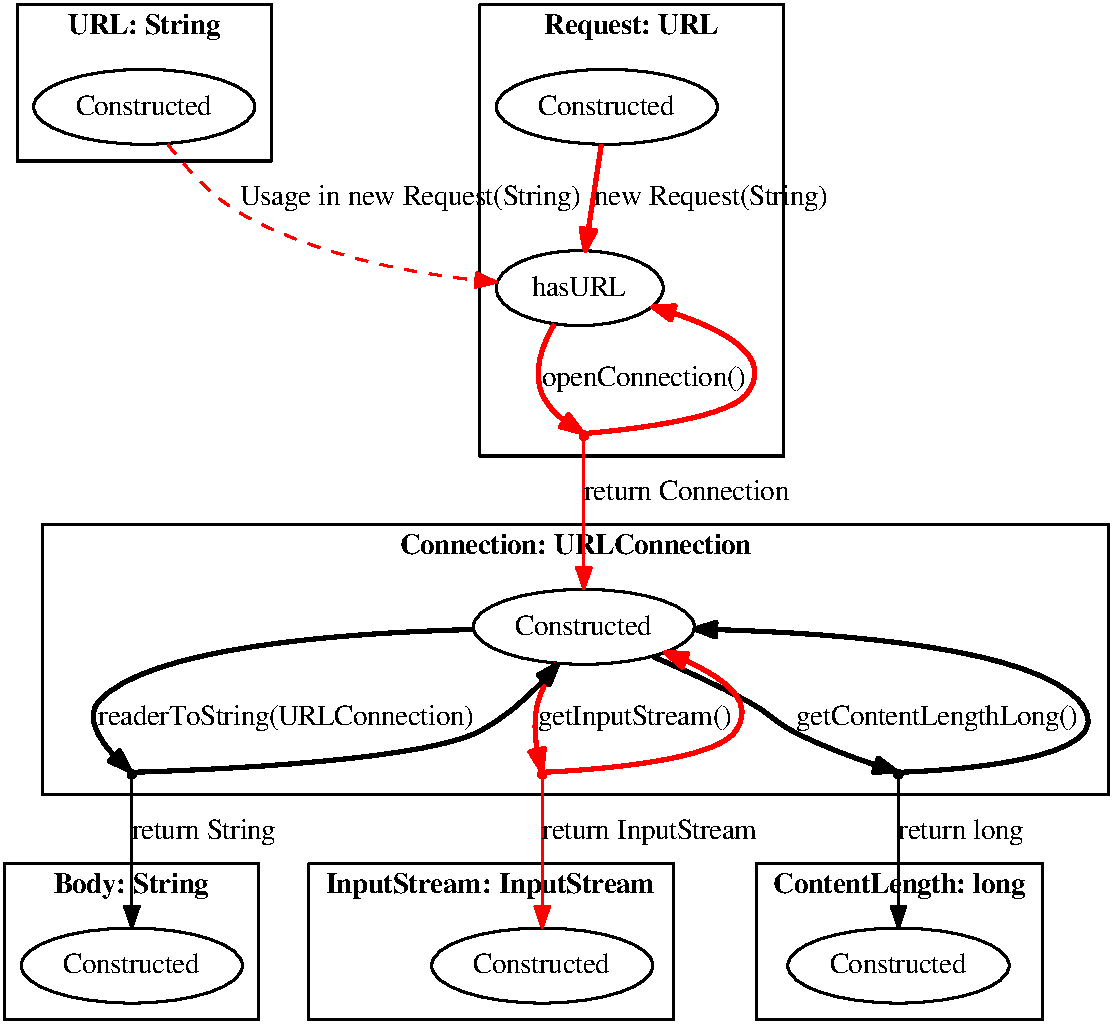
\includegraphics[width=0.75\textwidth]{javaPath-cropped.pdf}
\end{center}
\end{frame}

%{
%\usebackgroundtemplate{%
%\tikz\node[opacity=0.4]{
\includegraphics[height=\paperheight,width=\paperwidth]{links.jpg}};}
%\begin{frame}{Анализ портируемой программы}
%  \begin{mybox}[]
%  \begin{itemize}
%  	\item Задача: Необходимо найти все участки портируемой программы, которые используют библиотеку, и найти соответствующие им переходы в автомате
%  	\item Простейший вариант: получаем AST портируемой программы, ищем в нем все вызовы библиотечных методов и по имени метода выбираем переход в автомате
%  	\item Проблема: не всегда, имея только AST, можно выбрать подходящий переход в автомате
%  \end{itemize}
%  \end{mybox}
%\end{frame}
%}

{
\usebackgroundtemplate{
\includegraphics[height=\paperheight,width=\paperwidth]{links.jpg};}
\begin{frame}{Анализ портируемой программы}
  \begin{mybox}[]
  \begin{itemize}
  	\item Задача: необходимо связать вызовы API библиотеки в портируемой программе и переходы в автомате
  	\item Простейший вариант решения: находим все вызовы библиотечных методов и по имени метода выбираем переход в автомате
  	\item Проблема: некоторую информацию практически невозможно получить из исходного кода
  \end{itemize}
  \end{mybox}
\end{frame}
}

{
\usebackgroundtemplate{
\includegraphics[height=\paperheight,width=\paperwidth]{links.jpg};}
\begin{frame}{Анализ портируемой программы}
	\begin{mybox}[]
	\begin{itemize}
	\item В дополнение можно использовать динамический анализ: программа инструментируется, составляется трасса выполнения, в которой фиксируется необходимая информация.
	\item Подразумевается, что у портируемой программы имеется достаточный набор тестов
	\end{itemize}
	\end{mybox}
\end{frame}
}

{
\usebackgroundtemplate{%
\tikz\node[opacity=0.3]{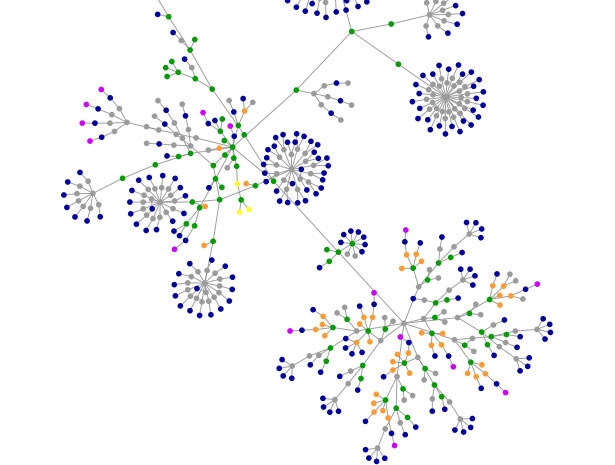
\includegraphics[height=\paperheight,width=\paperwidth]{chain.jpg}};}
\begin{frame}{Поиск соответствия между переходами}
  \begin{mybox}[]
  \begin{itemize}
  \item Задача: для каждого перехода в исходном автомате найти соответствующий ему набор переходов в целевом автомате
  \item Часто одному переходу в исходном автомате соответствуют несколько в целевом, и наоборот
  \item Критерий соответствия между переходами:
  \begin{itemize}
 	  	\item Сохраняются те же побочные эффекты
 	  	\item Порождается тот же набор сущностей
  \end{itemize}
  \end{itemize}
  \end{mybox}
\end{frame}
}

\begin{frame}[t]{Поиск соответствия между переходами}
\begin{picture}(320,250)
\put(0,130){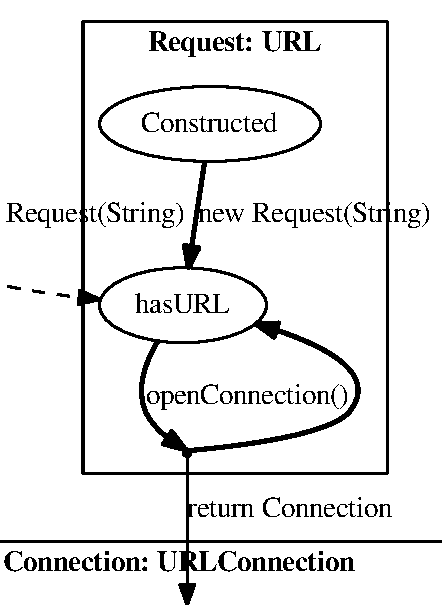
\includegraphics[width=0.3\textwidth]{java-element.pdf}}
\put(110,50){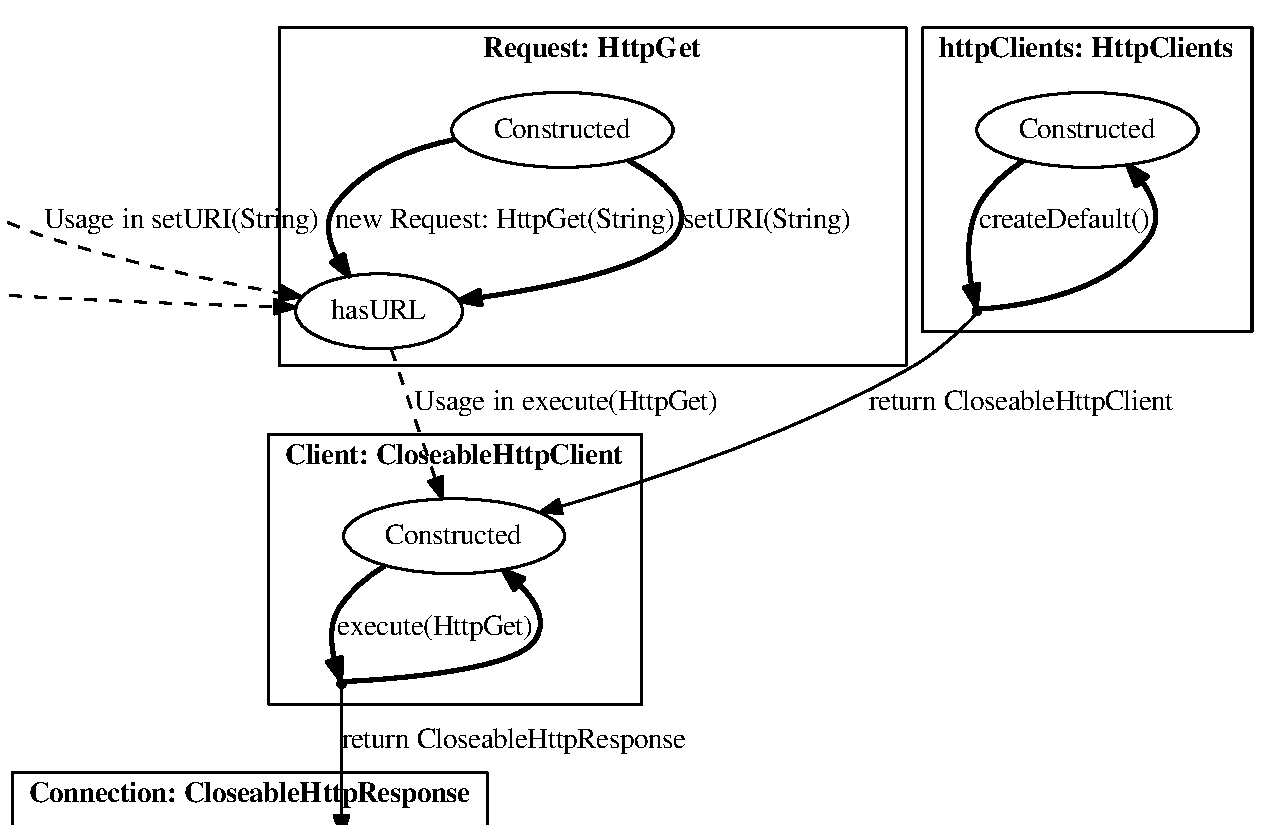
\includegraphics[width=0.7\textwidth]{apache-element.pdf}}
\put(100,170){$\Longrightarrow$}
\end{picture}
\end{frame}

{
\usebackgroundtemplate{%
\tikz\node[opacity=0.3]{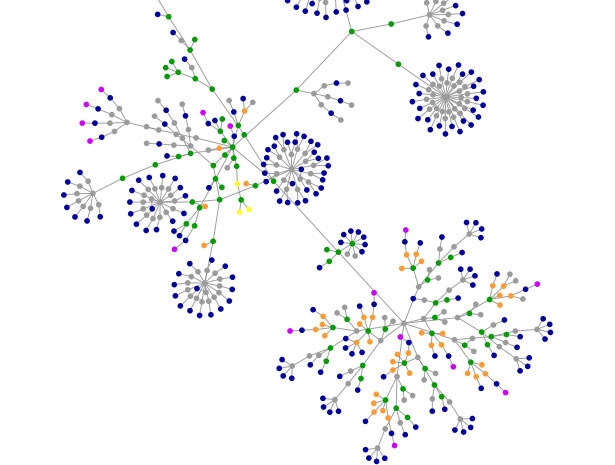
\includegraphics[height=\paperheight,width=\paperwidth]{chain.jpg}};}
\begin{frame}{Поиск соответствия между переходами}
  \begin{mybox}[]
  \begin{itemize}
   	\item Изначальный подход 
   	\begin{itemize}
   	\item модель переводится в граф и задача сводится к поиску пути на графе
   	\item \textcolor{red}{!} не учитываются побочные эффекты и условия переходов
   	\end{itemize}
   	
    \item Текущий подход: 
    \begin{itemize}
    \item из-за требования сохранить побочные эффекты, обычный граф не подходит
    \item сеть автоматов сводится к графу с атрибутами 
    \item используется модифицированный волновой алгоритм (учитывающий побочные эффекты)
    \end{itemize}
  \end{itemize}
  \end{mybox}
\end{frame}
}

%{
%\usebackgroundtemplate{%
%\tikz\node[opacity=0.3]{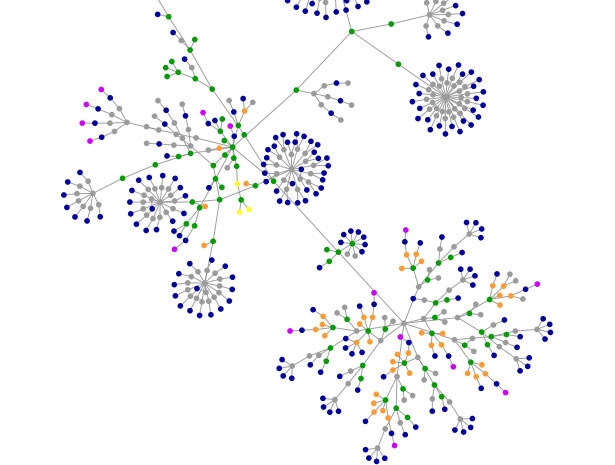
\includegraphics[height=\paperheight,width=\paperwidth]{chain.jpg}};}
%\begin{frame}{Поиск соответствия между моделями}
%  \begin{mybox}[]
%  Зависимости по данным:
%  \begin{itemize}
%    \item Сущности, которые необходимы для осуществления перехода (например, аргументы функции), отмечены в модели специальными связями
%  	\item Если для перехода требуется сущность, которая отсутствует в текущем контексте, ищется способ создания этой сущности
%  \end{itemize}
%  \end{mybox}
%\end{frame}
%}

%{
%\usebackgroundtemplate{%
%\tikz\node[opacity=0.3]{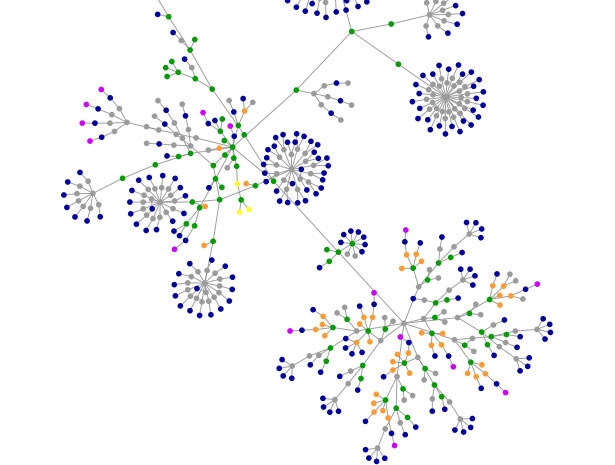
\includegraphics[height=\paperheight,width=\paperwidth]{chain.jpg}};}
%\begin{frame}{Применение изменений к коду}
%	\begin{mybox}[]
%  \begin{itemize}
%  	\item Для получения AST используется библиотека JavaParser
%  	\item Поддерживается синтаксис Java 8
%  	\item Измененный код компилируется и запускается
%  \end{itemize}
%\end{mybox}
%\end{frame}
%}

{
\usebackgroundtemplate{
\includegraphics[height=\paperheight,width=\paperwidth]{todolist.jpg};}
\begin{frame}{Прототип инструмента}
  \begin{mybox}[]
  Рассмотренные идеи реализуются в прототипе инструмента миграции для языка Java:
  \begin{itemize}
  	\item сформирован DSL на Kotlin для описания моделей библиотек
  	\item реализовано получение трассы выполнения мигрируемой программы (с использованием AspectJ)
  	\item производится портирование простых искусственных программ
  	\item создается система проверки корректности преобразования
  \end{itemize}
  \end{mybox}
\end{frame}
}

\begin{frame}[fragile]{Фрагмент DSL-описания модели библиотеки}
\begin{minted}[breaklines,fontsize=\scriptsize]{kotlin}
val url = StateMachine(entity = HTTPEntities.url)
val request = StateMachine(entity = HTTPEntities.request)
val connection = StateMachine(entity = HTTPEntities.connection)
val hasURL = State(name = "hasURL", machine = request)
ConstructorEdge(
     machine = request,
     src = request.getDefaultState(),
     dst = hasURL,
     param = listOf(Param(machine = url))
)
makeLinkedEdge(
    machine = request,
    src = hasURL,
    dst = connection.getDefaultState(),
    methodName = "openConnection"
)
\end{minted}
\end{frame}

\begin{frame}{Пример автомата}
	\begin{center}
		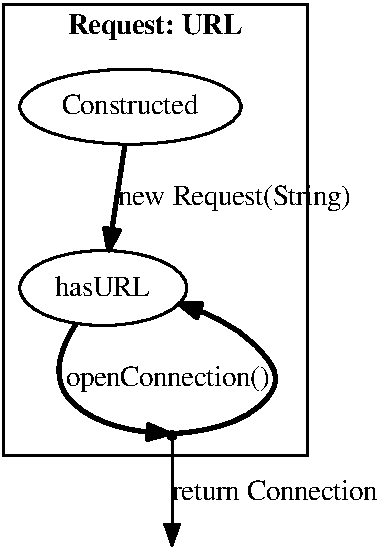
\includegraphics[height=0.9\textheight]{javaSmall-cropped.pdf}
	\end{center}
\end{frame}

\begin{frame}[fragile]{Пример миграции. Программа <<До>>}

\begin{minted}[breaklines,fontsize=\footnotesize]{java}
URL url = new URL("http://api.ipify.org/");
URLConnection conn = url.openConnection();
if (conn.getContentLengthLong() > 0) {
    String response = new BufferedReader(new InputStreamReader(conn.getInputStream()))
    .lines().collect(Collectors.joining("\n"));
    System.out.println(response);
} else {
    System.out.println("Error!");
}
\end{minted}
\end{frame}

\begin{frame}[fragile]{Результат миграции. Программа <<После>>}
\begin{minted}[breaklines,fontsize=\scriptsize]{java}
HttpGet url = new HttpGet("http://api.ipify.org/");
CloseableHttpClient newMachine_Client_0 = HttpClients.createDefault();
CloseableHttpResponse conn = newMachine_Client_0.execute(url);
long linkedEdge_ContentLength_1 = conn.getEntity().getContentLength();
if (linkedEdge_ContentLength_1 > 0) {
    InputStream linkedEdge_InputStream_2 = conn.getEntity().getContent();
    String response = new BufferedReader(new InputStreamReader(linkedEdge_InputStream_2))
    .lines().collect(Collectors.joining("\n"));
    System.out.println(response);
} else {
    System.out.println("Error!");
}
\end{minted}
\end{frame}

{
\usebackgroundtemplate{
\includegraphics[height=\paperheight,width=\paperwidth]{todolist.jpg};}
\begin{frame}{Дальнейшее развитие подхода}
	\begin{mybox}[]
	\begin{itemize}	
		\item Развитие метода поиска соответствия между автоматами
		\item Разработка метода сопоставления побочных эффектов
		\item ...
	\end{itemize}
	
	  \noindent\rule{4cm}{0.4pt}
	  
	  \begingroup
	  \tiny
	    	* В процессе обсуждения
	  \endgroup
	\end{mybox}
\end{frame}
}

{
\usebackgroundtemplate{
\includegraphics[height=\paperheight,width=\paperwidth]{todolist.jpg};}
\begin{frame}{Дальнейшее развитие прототипа инструмента}
	\begin{mybox}[]
	\begin{itemize}
		\item Проектирование языка для описания моделей (сейчас это ad-hoc решение)
		\item Расширение поддержки модели в прототипе
		\item (Cущественное) пополнение репозитория моделей библиотек
		\item Создание репозитория тестовых программ для миграции
		\item Тестирование инструмента на реальных проектах
	\end{itemize}
	\end{mybox}
\end{frame}
}

\begin{frame}[t]{Контакты}
	Email: aleksyuk@kspt.icc.spbstu.ru
	
	Github: \url{https://github.com/h31/LibraryMigration}
	
	\vspace{1cm}
	\begin{center}
		\Large
		Спасибо за внимание!
	\end{center}
\end{frame}

\end{document}
